% Generated by analysis/plot_results.py; edit that file to regenerate.
\centering

\includegraphics[width=1.0000\linewidth]{figures/data_app_localization_legend.pdf}
\par\vspace{1pt}
\begin{subfigure}[t]{0.3260\linewidth}
\centering
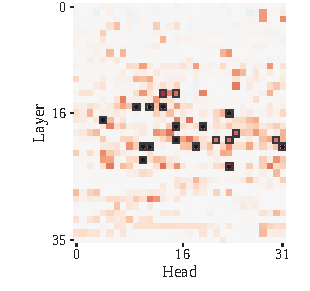
\includegraphics[width=\linewidth]{figures/data_app_localization_a.pdf}
\caption{Qwen3-4B}
\label{fig:data-app-localization-a}
\end{subfigure}%
\hfill%
\begin{subfigure}[t]{0.3260\linewidth}
\centering
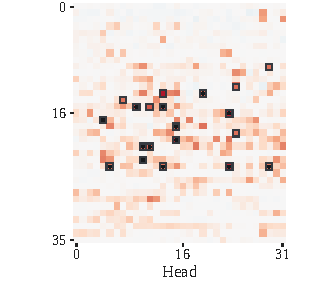
\includegraphics[width=\linewidth]{figures/data_app_localization_b.pdf}
\caption{Qwen3-8B}
\label{fig:data-app-localization-b}
\end{subfigure}%
\hfill%
\begin{subfigure}[t]{0.3260\linewidth}
\centering
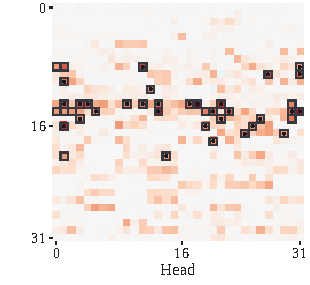
\includegraphics[width=\linewidth]{figures/data_app_localization_c.pdf}
\caption{Llama-3.1-8B}
\label{fig:data-app-localization-c}
\end{subfigure}%
\par
\par\vspace{2pt}
\begin{subfigure}[t]{0.3260\linewidth}
\centering
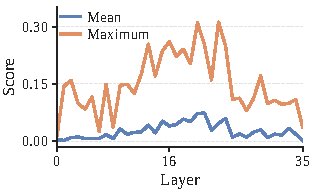
\includegraphics[width=\linewidth]{figures/data_app_localization_d.pdf}
\caption{Qwen3-4B: layer profile}
\label{fig:data-app-localization-d}
\end{subfigure}%
\hfill%
\begin{subfigure}[t]{0.3260\linewidth}
\centering
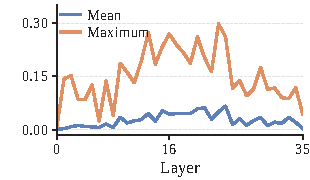
\includegraphics[width=\linewidth]{figures/data_app_localization_e.pdf}
\caption{Qwen3-8B: layer profile}
\label{fig:data-app-localization-e}
\end{subfigure}%
\hfill%
\begin{subfigure}[t]{0.3260\linewidth}
\centering
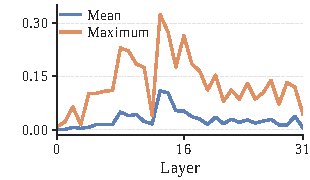
\includegraphics[width=\linewidth]{figures/data_app_localization_f.pdf}
\caption{Llama-3.1-8B: layer profile}
\label{fig:data-app-localization-f}
\end{subfigure}%
\par
